\documentclass[journal,12pt,onecolumn]{IEEEtran}
\usepackage{mathtools,amssymb,amsfonts}
\usepackage{algorithmic}
\usepackage{algorithm}
\usepackage{graphicx}
\usepackage{xcolor}
\usepackage{float}
\usepackage{setspace}
\usepackage{subcaption}
\usepackage[hidelinks]{hyperref}
\usepackage{multirow}

\doublespacing

\hypersetup{
   colorlinks=true,
   linkcolor=blue,
   citecolor=black,
   urlcolor=blue
}

\usepackage{titlesec}
\titlespacing*{\section}{0pt}{12pt plus 4pt minus 2pt}{12pt plus 2pt minus 2pt}
\titlespacing*{\subsection}{0pt}{12pt plus 4pt minus 2pt}{8pt plus 2pt minus 2pt}
\titlespacing*{\subsubsection}{0pt}{12pt plus 4pt minus 2pt}{6pt plus 2pt minus 2pt}

\title{Evolutionary Computing: Comprehensive Review}
\author{
   \IEEEauthorblockN{Matthew D. Branson} \\
   \IEEEauthorblockA{\textit{Department of Computer Science} \\
   \textit{Missouri State University}\\
   Springfield, MO \\
   branson773@live.missouristate.edu
   }
}

\date{July 16, 2025}

\begin{document}

\maketitle

\begin{abstract}
This paper presents a comprehensive review of key topics in evolutionary computing, including genetic algorithms, multi-objective optimization, genetic programming, neuroevolution, and co-evolution.
\end{abstract}

\begin{IEEEkeywords}
Genetic algorithms, multi-objective optimization, genetic programming, neuroevolution, NEAT, co-evolution
\end{IEEEkeywords}

% Section A
\section{Genetic Algorithms}

\subsection{Selection Pressure}

Selection pressure controls how strongly fitness differences influence reproduction probability in genetic algorithms, balancing exploration of new solutions against exploitation of good ones. Too high pressure causes premature convergence: superior individuals dominate reproduction, rapidly eliminating diversity and trapping populations in local optima. Too low pressure degenerates into random search: beneficial traits spread slowly or not at all, wasting computation on inferior solutions.

Roulette wheel selection creates pressure proportional to fitness ratios through $p_i = f_i / \sum f_j$. This dependence on fitness distribution causes unpredictable behavior: when fitness values vary widely, small differences become exaggerated; when compressed, important distinctions disappear. Selection pressure fluctuates throughout evolution as the population's fitness profile changes. Tournament selection provides consistent control via tournament size $k$: randomly select $k$ individuals, choose the best. Pressure depends only on rank, not absolute fitness. Larger $k$ increases pressure predictably ($k=2$ for diversity preservation, $k=7$ for near-deterministic selection).

\subsection{Premature Convergence}

Binary-encoded GAs converge prematurely when populations lose diversity before finding global optima. High selection pressure rapidly fixes early good solutions, while small populations lack diversity for thorough exploration. The Hamming cliff problem worsens this: single bit flips can cause large phenotypic jumps, preventing gradual improvement. Binary encoding creates deceptive building blocks where good partial solutions combine poorly. Once converged, crossover between similar individuals yields near-identical offspring, and mutation alone cannot efficiently escape local optima.

Effective mitigation strategies include diversity preservation and adaptive parameter control. Fitness sharing divides populations into niches by penalizing individuals in crowded regions, maintaining exploration across multiple search space areas. Speciation groups genetically similar individuals and restricts competition within groups, protecting innovative solutions from premature elimination. Adaptive parameter control dynamically adjusts selection pressure and mutation rates based on population diversity metrics: reducing selection pressure when diversity drops below thresholds, or increasing mutation rates from the standard 1/L to reintroduce variation. Random restarts detect convergence through diversity metrics or fitness stagnation, then reinitialize portions of the population while preserving elite solutions. These strategies can be combined: maintaining diverse subpopulations while adapting parameters ensures continued exploration without sacrificing exploitation of promising regions.

% Section B
\section{Multi-Objective Optimization}

\subsection{Pareto Dominance and Pareto Optimality}

Pareto dominance creates partial ordering in multi-objective space: solution $\mathbf{x}$ dominates $\mathbf{y}$ ($\mathbf{x} \succ \mathbf{y}$) when $\mathbf{x}$ equals or betters $\mathbf{y}$ in all objectives and strictly betters it in at least one. For minimization: $\forall i: f_i(\mathbf{x}) \leq f_i(\mathbf{y})$ and $\exists j: f_j(\mathbf{x}) < f_j(\mathbf{y})$. Pareto optimality characterizes non-dominated solutions: those that cannot improve any objective without degrading another. The Pareto-optimal set contains all such solutions; its objective space image forms the Pareto front.

Figure~\ref{fig:pareto_dominance} illustrates cantilever beam design minimizing weight and deflection. Solutions A (0.5kg, 2.0mm) and E (3.0kg, 1.75mm) are mutually non-dominated since each excels in one objective. The circled solutions form the Pareto front representing optimal trade-offs. Figure~\ref{fig:moo_space_to_front} shows how feasible designs filter down to this optimal boundary where no solution can improve without sacrifice.

\begin{figure}[h]
\centering
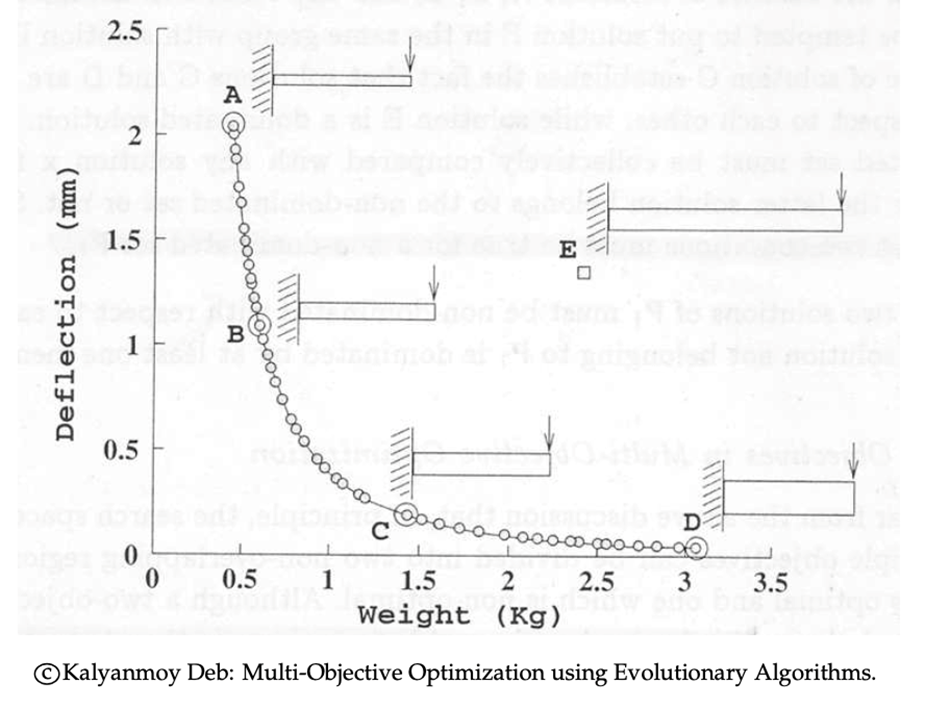
\includegraphics[width=0.8\textwidth]{moo_pareto_dominance.png}
\caption{Cantilever beam design trade-offs. Points A-E show different beam configurations. The circled solutions form the Pareto-optimal front where no improvement in one objective is possible without degrading the other.}
\label{fig:pareto_dominance}
\end{figure}

\begin{figure}[h]
\centering
\begin{subfigure}[b]{0.48\textwidth}
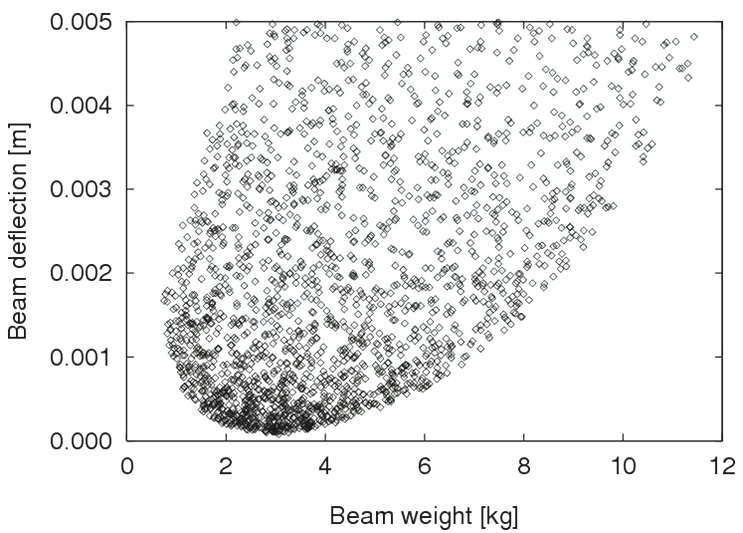
\includegraphics[width=\textwidth]{moo_feasible_space.png}
\caption{Complete feasible solution space}
\label{fig:moo_feasible}
\end{subfigure}
\hfill
\begin{subfigure}[b]{0.48\textwidth}
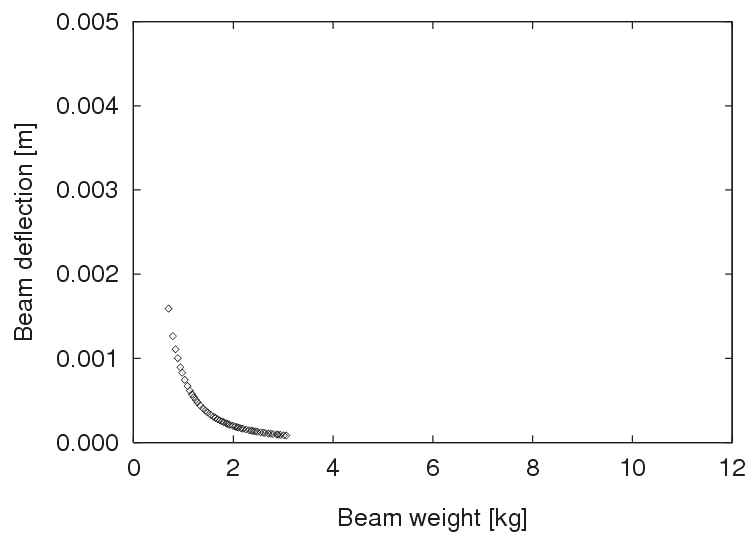
\includegraphics[width=\textwidth]{moo_pareto_front.png}
\caption{Extracted Pareto-optimal front}
\label{fig:moo_front}
\end{subfigure}
\caption{From many feasible cantilever designs to the Pareto-optimal subset}
\label{fig:moo_space_to_front}
\end{figure}

\subsection{Diversity Preservation}

Diversity preservation ensures MOEAs approximate entire Pareto fronts rather than clustering in easily-found regions. Without diversity mechanisms, populations miss critical trade-offs and converge prematurely. NSGA-II's crowding distance exemplifies effective preservation: calculating half the perimeter of cuboids formed by neighboring solutions, then favoring sparse-region solutions during selection. This metric-free approach automatically adapts to different objective scales and Pareto front geometries. Diversity preservation serves three purposes: providing complete trade-off information for decision-making, preventing premature convergence to suboptimal regions, and maintaining genetic variation for continued exploration.

\subsection{Limitations}

Weighted sum scalarization $f = \sum w_i f_i$ fails on non-convex Pareto fronts because it creates linear level sets (hyperplanes) in objective space. Consider transportation modes minimizing cost and time: air (high cost, low time) and sea (low cost, high time) might connect convexly, but rail creating a concave indentation remains unreachable by any weight combination. The hyperplane cannot penetrate concave regions regardless of weights chosen. Additional limitations include requiring a priori weight specification before seeing trade-offs, and non-uniform solution distribution where equal weight spacing produces unequal Pareto front coverage. Small weight changes may cause large solution jumps or no change depending on front geometry.

% Section C
\section{Genetic Programming}

\subsection{Comparing Genetic Programming and Genetic Algorithms}

Representation distinguishes GP from GA fundamentally. GP evolves variable-size tree structures where internal nodes are functions and leaves are terminals, encoding programs like $(+ \; x \; (* \; 2 \; y))$ for $x + 2y$. Trees grow, shrink, and reshape during evolution. GA evolves fixed-length linear chromosomes: binary strings, real vectors, or integer arrays that maintain constant size throughout evolution.

Operators reflect structural differences. GP crossover exchanges entire subtrees between parents, dramatically altering program size and behavior by swapping complex branches for simple terminals. GP mutation replaces subtrees or changes node operations. GA crossover operates positionally (one-point, two-point, uniform), exchanging corresponding segments. GA mutation flips bits or perturbs values within fixed positions. These operational differences stem from GP's variable structure versus GA's fixed encoding.

Application domains exploit representational strengths. GP excels when solution structure is unknown: symbolic regression discovering mathematical formulas, automatic programming, circuit design creating novel topologies. NASA's evolved antenna exemplifies GP finding non-intuitive structures humans wouldn't conceive. GA dominates parameter optimization within known structures: neural network weights, robot parameters (leg count, sensor positions), combinatorial problems (TSP, scheduling, N-Queens).

\subsection{Closure and Sufficiency}

Closure ensures any function can accept any function or terminal output as input, preventing runtime errors when crossover creates new program combinations. Without closure, evolved programs crash when incompatible types connect. Protected operators enforce closure: division returning 1 for divide-by-zero maintains numeric consistency. Sufficiency ensures the primitive set can express target solutions without unnecessary bloat. Insufficient primitives make solutions impossible; excess primitives expand search space wastefully.

Consider symbolic regression for $f(x) = x^2 + x + 1$: Function set $\{+, -, *, /\}$ (protected division) with terminal set $\{x, \mathcal{R}\}$ (ephemeral constants) satisfies both properties. Closure holds because all operations accept and return real numbers, with $a / 0 = 1$ preventing errors. Sufficiency confirmed by expressing the target as $(+ \; (+ \; (* \; x \; x) \; x) \; 1)$. For robot control: Functions $\{\text{IF\_SENSOR}, \text{PROGN2}, \text{TURN}, \text{MOVE}\}$ with terminals $\{\text{LEFT}, \text{RIGHT}, \text{FORWARD}, \text{SENSOR\_READING}\}$ maintain closure through consistent action/value types while providing sufficient expressiveness for navigation tasks. NASA's antenna evolution succeeded using $\{\text{forward}(L,R), \text{rotate\_x}(\theta), \text{rotate\_y}(\theta), \text{rotate\_z}(\theta)\}$, maintaining closure (all produce valid antenna segments) with sufficient expressiveness for complex 3D structures.

% Section D
\section{Neuroevolution}

\subsection{NeuroEvolution of Augmenting Topologies}

NEAT's three key innovations enable simultaneous evolution of neural network topology and weights. Historical markings assign each new gene a global innovation number persisting throughout evolution. During crossover, genes align by these markers rather than position, enabling meaningful structure exchange between different topologies. This solves the competing conventions problem where identical networks have different encodings. Speciation protects topological innovations by grouping genomes using compatibility distance: $\delta = \frac{c_1 E}{N} + \frac{c_2 D}{N} + c_3 \bar{w}$, where $E$ = excess genes, $D$ = disjoint genes, $\bar{w}$ = average weight differences, $N$ = normalization. Genomes within threshold $\delta_t$ form species, competing primarily within niches. Complexification starts with minimal topologies (often direct input-output connections) and incrementally adds structure through mutations that insert nodes or connections.

\subsection{Comparison with Fixed Topology Neuroevolution}

Fixed-topology neuroevolution predefines network architecture, evolving only weights within an $n$-dimensional space. Practitioners must guess network size: too small limits expressiveness, too large wastes computation. Standard GA operators apply directly to weight vectors. NEAT evolves both topology and weights, automatically discovering minimal sufficient architectures. Networks start simple and grow as needed. This requires specialized operators: structural mutations add/remove components, crossover aligns by historical markers not position.

Dynamic environments reveal topology evolution's advantages. When environments change, computational requirements shift: new sensors activate, different behaviors emerge. Fixed topologies can only reweight existing connections while NEAT grows new pathways or prunes obsolete structures. The fundamental difference is that NEAT explores the space of all possible topologies and their weights, enabling discovery of innovative architectures impossible within predetermined structures.

\subsection{Speciation}

Speciation protects innovation because new topological features rarely improve fitness immediately. Additional nodes or connections increase complexity without refined functionality, making them vulnerable to elimination by established, optimized networks. Without protection, populations converge to variations of early topologies, missing superior architectures.

Implementation clusters genomes by compatibility distance $\delta = \frac{c_1 E}{N} + \frac{c_2 D}{N} + c_3 \bar{w}$ with coefficients balancing topology versus weight importance. Genomes join the first species where $\delta < \delta_t$ or found new species. Fitness sharing divides fitness by species size, preventing domination. Selection occurs within species, not globally.

Without speciation, innovation suffocates as new structures cannot compete with optimized solutions. Competing conventions proliferate when multiple encodings of similar networks coexist, making crossover destructive. Populations lose diversity to escape local optima requiring coordinated changes. Protected innovation within niches enables gradual optimization of novel structures that eventually surpass established solutions.

% Section E
\section{Co-Evolution}

\subsection{Cooperative vs. Competitive Co-Evolution}

Cooperative co-evolution achieves fitness through synergy: components succeed together or fail together. Competitive co-evolution achieves fitness through superiority: success requires defeating opponents. In cooperative systems, populations evolve complementary specializations converging toward stable roles. In competitive systems, populations engage in arms races that may never stabilize.

Soccer team evolution exemplifies cooperation: separate populations evolve goalkeepers, defenders, midfielders, and forwards. Each position's fitness depends on team performance. A brilliant forward cannot succeed with poor defenders. The challenge is credit assignment: determining individual contributions to team success. Without careful design, one exceptional player dominates evaluations while others drift randomly.

Sorting algorithm evolution demonstrates competition: one population evolves algorithms, another evolves test cases. Algorithms gain fitness by correctly sorting sequences; test cases gain fitness by stumping algorithms. This creates escalating pressure where algorithms become more robust, test cases become more pathological, and neither population reaches a stable optimum as each improvement forces counter-adaptation.

\subsection{The Red Queen Effect}

The Red Queen effect describes evolutionary treadmills where populations must continuously evolve to maintain relative fitness. Named after Carroll's character who runs constantly to stay in place, it captures how improvement yields no advantage when opponents improve equally. Predator-prey dynamics exemplify this: faster rabbits force evolution of faster foxes, which select for even faster rabbits.

In competitive co-evolution, this prevents traditional convergence. Fixed-landscape optimization climbs toward stable peaks, but competitive landscapes shift with opponent evolution. A chess program maintaining 1500 ELO may dramatically improve in absolute strength while its relative performance stays constant. The Lotka-Volterra equations model these dynamics: $\frac{dx}{dt} = \alpha x - \beta xy$ and $\frac{dy}{dt} = -\gamma y + \delta xy$ produce coupled oscillations without equilibrium. Populations may cycle indefinitely: strategy A beats B, B beats C, C beats A. Arms races force perpetual innovation as each adaptation triggers counter-adaptation.

\subsection{Challenges in Co-Evolution}

Co-evolutionary fitness evaluation faces fundamental challenges because performance depends on interaction partners. Relative fitness measures performance against current populations: a chess player's strength depends entirely on opponents faced. This creates transitivity failures (A beats B beats C beats A), temporal inconsistency (today's champion loses to yesterday's mediocre player after adaptation), and computational expense (each evaluation requires multiple interactions). Populations may improve dramatically while maintaining identical relative rankings.

Absolute fitness uses fixed benchmarks: chess programs play standard opponents, sorting algorithms face predetermined tests. This enables progress tracking but suffers from benchmark overfitting and misses failure modes that adaptive opponents would expose. Static tests cannot capture co-evolutionary diversity.

\end{document}